\section{Introduction}

\begin{frame}[plain]
  \begin{tikzpicture}[remember picture,overlay]
    \node[at=(current page.center)] {
      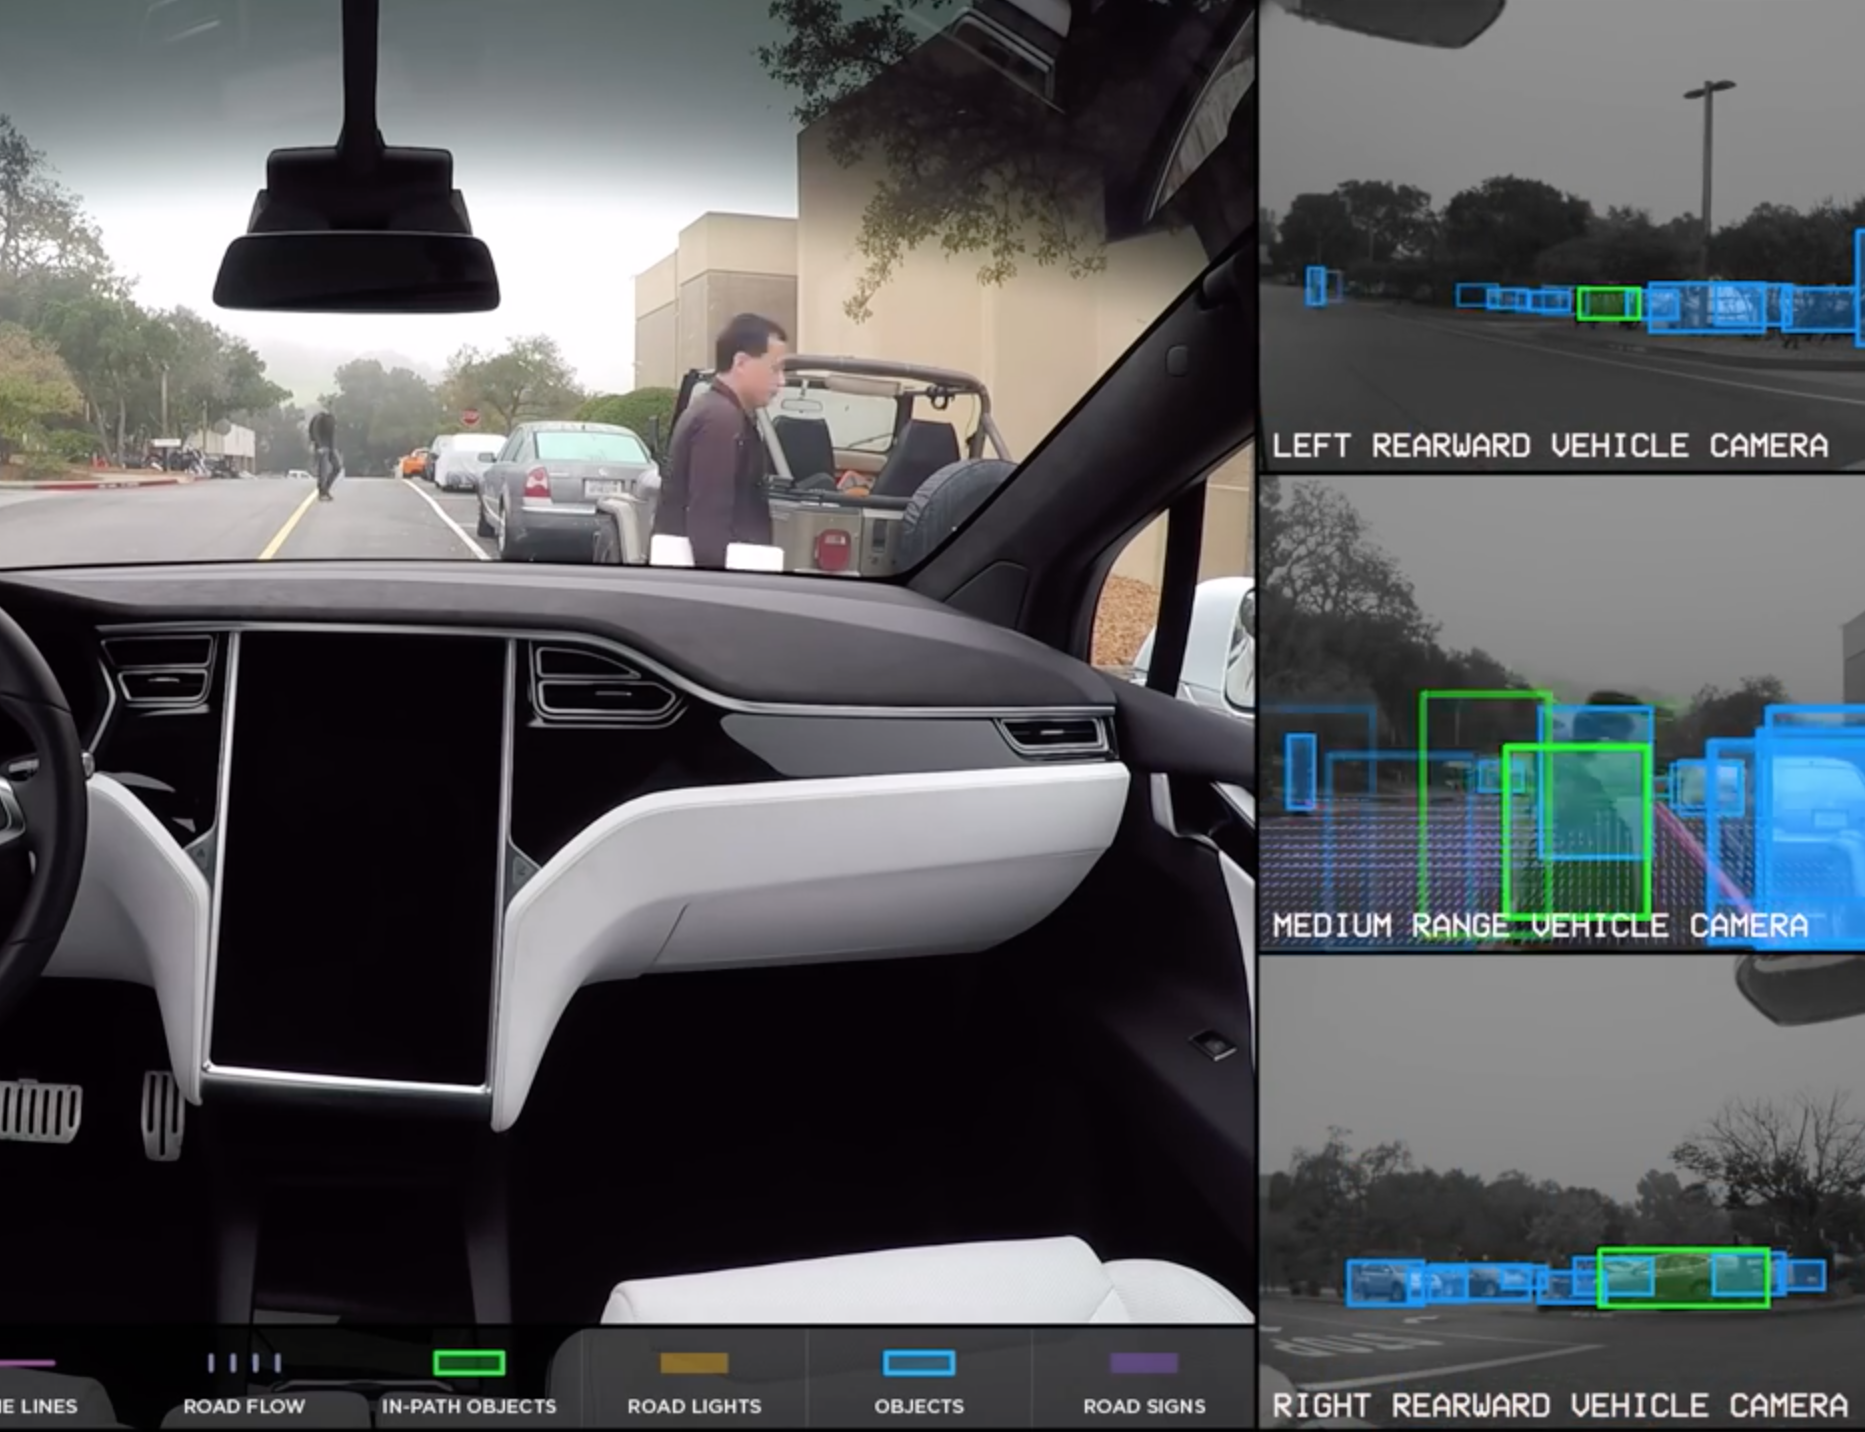
\includegraphics[width=\paperwidth]{intro_tesla.png}
    };
  \end{tikzpicture}
\end{frame}

\begin{frame}{Image Classification Pipeline}
\centering
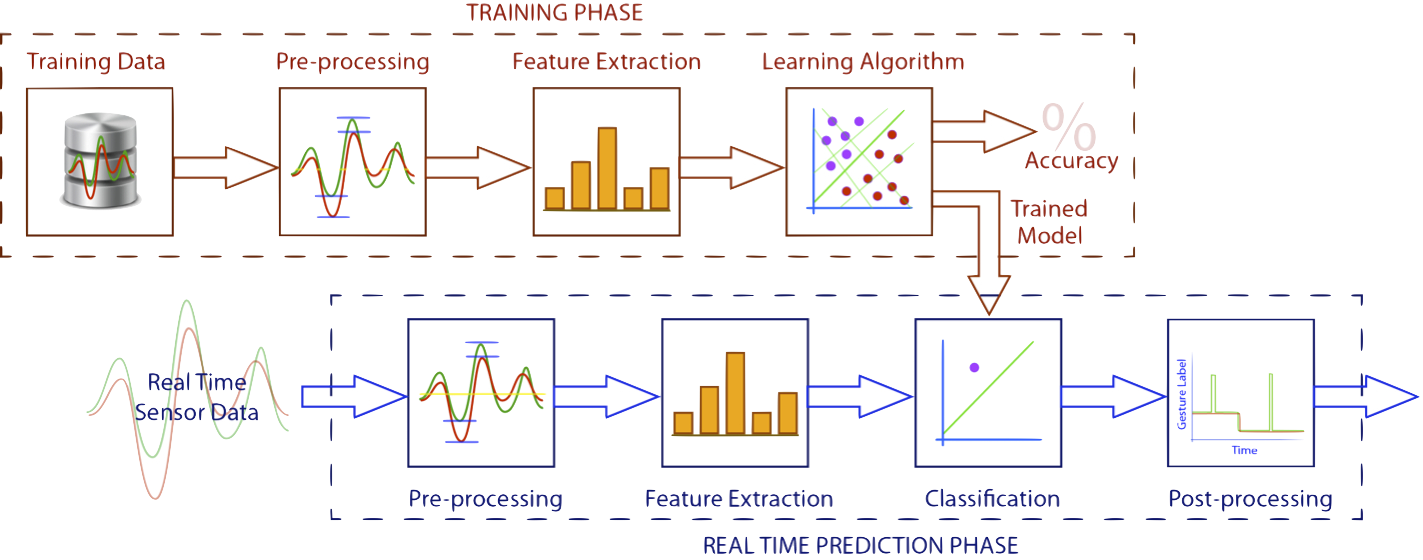
\includegraphics[width=\textwidth]{pipeline_configuration.png}\\
\small
Classic pipeline for \textbf{Pedestrian Detection}
\end{frame}

\begin{frame}{1. Region Proposal}

Analyzes the entire frame and tries to
\begin{itemize}
  \item discard most of the negative regions
  \item extract all the positive regions
\end{itemize}
\vspace{1mm}
Strong influence on
\begin{itemize}
  \item computational efficiency
  \item task accuracy
\end{itemize}
\end{frame}

\begin{frame}{1. Region Proposal}

\only<1>{
\textbf{Sliding window:}
\begin{itemize}
  \item Simple and suitable for multiple scales
  \item Scans the frame horizontally and vertically with a shifting window
  \item Yields a very large number of regions
  \item Inefficient
\end{itemize}
}


\only<2>{
\small
\textbf{Selective search:}
\begin{itemize}
  \item More complex
  \item Smaller number of candidate regions
  \item Reduces the computational burden
\end{itemize}
}
\pause
\only<2>{
\small
\textbf{Locally Decorrelated Channel Features (LDCF):}
\begin{itemize}
  \item Ad-hoc pedestrian detection algorithm
  \item Candidate region with a confidence value
  \item Tradeoff between precision and recall
\end{itemize}
}

\end{frame}


\begin{frame}{2. Feature Extraction}
\textbf{Input}: candidate regions\\
\textbf{Output}: feature vector (set of real or binary values)\\
Examples: HOG, CNN, Integral Channel Features
\end{frame}

\begin{frame}{3. Classification}
\textbf{Input}: feature vector (set of real or binary values)\\
\textbf{Output}: final binary response\\
Examples: Adaboost, SVM, cross-entropy based loss functions
\end{frame}
